\chapter{Implementation}

Precise documentation of the program comes in form of JavaDoc as well. Here we will mention the most important actors concepts or approaches.

\section{ER/Studio}

\subsection{File Reverse-Engineering Tool}
\label{subsec:dm1_tool}

We need to decrypt relations between tables in ER/Studio .DM1 files in order to be able to deconstruct objects stored in the files. 
We described the file format together with the need for help in \autoref{subsec:dm1_format}.
The task is to find out what links are leading between tables in the format. The links are done via primary and foreign keys.

Input is an arbitrary .DM1 file and output must describe the logical layout. 
We proposed the parallel with relational databases which can be represented understandably by a relational diagram, we will try to visualize the result showing organization of the format by such diagram. 
For creation of relational diagram a modeling tools are used. 
If we are able to generate a SQL code definition of the file format enriched with definition of primary and foreign keys, modeling tools can transform such code into a visual representation of database structure that is creates.

Modeling tools commonly have the ability of reverse engineer a database, however they do it based on metadata from a deployed database where keys are defined. 
If we just described tables in .DM1 file format by SQL creates, there is no tool that could effectively infer relations. That is why we need this reverse-engineering tool.
As the development of such tool is not the focal point of the work, this will be not an out-box general solution for deducing keys for relational databases, but will provide a basic overview of .DM1 file organization. Also it is not a complete solution but is primarily aimed on the objects and properties we picked by analysis described above in \autoref{metadata_enumeration}.

The decision what programming language should be used for the discussed utility fell to Java as the final Metadata Extractor was going to be written in the language and there are units we want to reuse in this tool as well as in further parts. Although there may be scripting languages that would make some operations, like joins on tables easier.
For example in order to go through the file format a parser is needed. Instead of writing it multiple times we will write it once in Java and use here just like in Metadata Extractor itself. \\

The idea is to look at the tables from two views.

The first one is to take into account only metadata which is represented by the class \classname{DependencyCreator}. It treats column that looks like keys (eg. those which name ends with "ID", the policy is determined by \methodname{isOnBlacklist} method) as the same across all tables. 
The main method here is createDependencies which pairs potential key columns and tables in what they are used.
Then there is the class \classname{RelationFinderByTableDefinitions} that allows querying over the structure found by \classname{DependecyCreator} showing what tables are possibly related through a series of joins.
Among other there is the general method \methodname{getDependenciesWithPaths} is showing a sequence of joins needed to do in order to put put together records from table a with those from table b.

The second view takes into account the data stored in tables as well. 
When analyzing what are relations between columns, we see a table as a collection of columns, where a column has a set of values. This way we can examine if columns with same names have similar contents.
In contrast when getting records from a table we see a collection of rows.
The \classname{RelationFinderByTableContents} class is used for the further search for key columns.

It filters tables that without content, thus irrelevant.
Has method for determining if a column can be considered a primary key of a table, that is when it contains only distinct ids.
Method for finding out if a column can be foreign key corresponding to primary key column, thus the first one contains subset of values for the other.
In .DM1 file format there is a table Identity Value that explicitly pairs tables with their primary keys. 
The class also inspects if the primary keys are defined in strict order or if there is some pattern key definitions follow.

The classes above are used for being able to look from multiple perspectives and to comprehend the format.
To put it all together and finally generate the desired output in form of a SQL definition of .DM1 tables in SQL with keys out of the analysis the class \classname{TablesToSQLConverter} is used.
The main method is \methodname{writeMySQLSource} that at first defines create table procedure for each table from ER/Studio source. 
Then the phase of creating key constraints takes place. It operates on candidate columns that satisfy policies in \classname{DepedencyCreator} to be key column and are present in at least one table so at least one join can be made using them.
There is also space for defining manually the knowledge we gained by inspecting the format using \classname{RelationFinder*} classes by inserting pairs table-primary keys.
So primary keys are defined from user-defined information, the information stored in Identity Value table and are inferred based on policies taking into account name of a column and name of the table it belongs to.
If a column is set as a primary key in one table for each of the remaining ones that contain it, it is marked as a foreign identifier.
In case there are columns that are candidates for being keys but no source table was assigned to them in previous steps one of the tables is chosen as the source, that may cause inaccuracies in the final result but the main message should not get lost.

\subsection{Parser}
\label{subsec:dm1_parser}

Existing CSV parsers are made to process a single CSV structure per file. There is no unified definition for the comma-separated-value files, but usually they do not allow naming CSV tables as present in .DM1 files.
What is important to say about CSV record is that each entry is on a located on a separate line, fields in an entry are separated by a comma, the last record is followed by line break. A field may contain a comma or line break but must be enclosed by quotes. 
If a double quote appears in a field, it must be in the enclosed section and the quote itself must be doubled. \cite{RfcCSV}

We know the structure we need to parse contains tables consisting of a name on a single line, definition of columns and entries. Two tables are separated by a single empty line.

Putting it all together it seems to be easier to come with an own parser for .DM1 files that processes the files into a set of tables identified by their names. 

To represent a single table we have the class \classname{CSVTable} which contains its name, definition of columns, in other words names for each of its properties \classname{CSVColumnDefinition}, and finally records themselves - instances of \classname{CSVColumn} which are contents of a table.

However, the view on a table may vary due to use of a parser. In the reverse-engineering tool we inspect what values are stored in a column, examine the domain of these values etc. That is the case when a table contents is for us set of columns. Whereas, if we see a table as set of records, each record having properties based on columns of the table, from this perspective a table is a set of rows. The second case is needed when reading the contents instead of inspecting relations between tables and columns.

Getting a name of a table is an easy job as its just a single textual line. To resolve a record is a slightly more challenging task. We designed an automaton that accepts well formed records of our CSV table.

We will propose a non-deterministic finite automaton, even though it can be translated to a deterministic one, we consider DFA being more clear and descriptive in this situation.
Set of states $Q = {I, Q, E, A, F}$
Alphabet $\sigma$ is a set of chars that can appear in a string as that is what the automaton processes and lambda.
Transitions are illustrated in the following figure.

\begin{figure}[H]
\begin{center}
	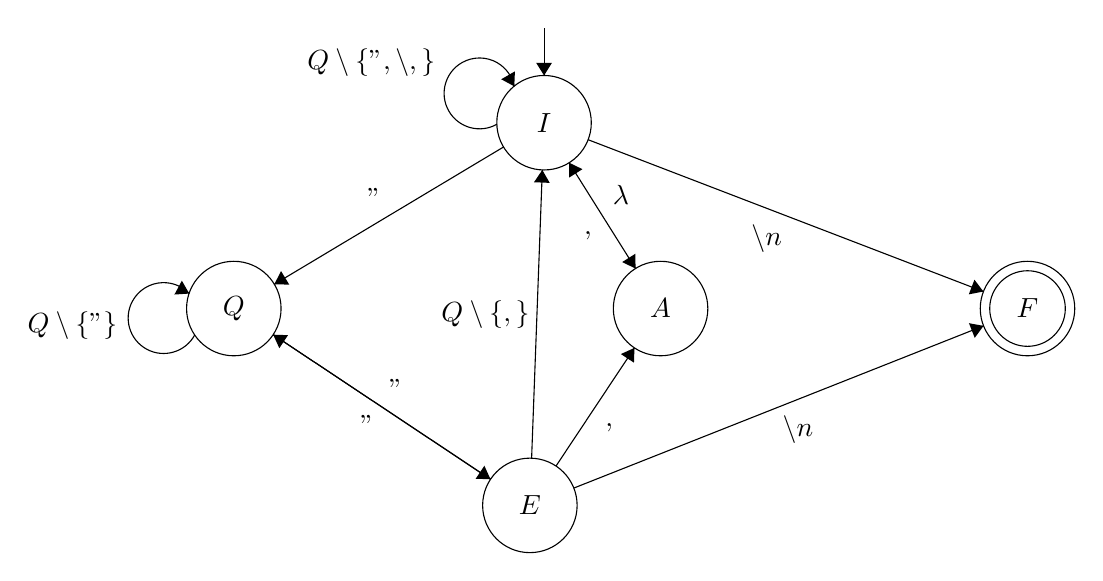
\begin{tikzpicture}[scale=0.2]
	\tikzstyle{every node}+=[inner sep=0pt]
	\draw [black] (40.8,-21.4) circle (3);
	\draw (40.8,-21.4) node {$I$};
	\draw [black] (71.5,-33.2) circle (3);
	\draw (71.5,-33.2) node {$F$};
	\draw [black] (71.5,-33.2) circle (2.4);
	\draw [black] (21.1,-33.2) circle (3);
	\draw (21.1,-33.2) node {$Q$};
	\draw [black] (48.2,-33.2) circle (3);
	\draw (48.2,-33.2) node {$A$};
	\draw [black] (39.9,-45.7) circle (3);
	\draw (39.9,-45.7) node {$E$};
	\draw [black] (40.8,-15.4) -- (40.8,-18.4);
	\fill [black] (40.8,-18.4) -- (41.3,-17.6) -- (40.3,-17.6);
	\draw [black] (37.813,-21.495) arc (299.55605:11.55605:2.25);
	\fill [black] (38.91,-19.09) -- (38.95,-18.14) -- (38.08,-18.64);
	\draw (33.93,-17.59) node [left] {$Q\setminus\left\{",\backslash,\right\}$};
	\draw [black] (43.6,-22.48) -- (68.7,-32.12);
	\fill [black] (68.7,-32.12) -- (68.13,-31.37) -- (67.77,-32.3);
	\draw (54.94,-27.83) node [below] {$\backslash n$};
	\draw [black] (38.23,-22.94) -- (23.67,-31.66);
	\fill [black] (23.67,-31.66) -- (24.62,-31.68) -- (24.1,-30.82);
	\draw (30.04,-26.8) node [above] {$"$};
	\draw [black] (18.622,-34.87) arc (-28.28273:-316.28273:2.25);
	\fill [black] (18.27,-32.25) -- (17.8,-31.43) -- (17.33,-32.31);
	\draw (13.73,-34.26) node [left] {$Q\setminus\left\{"\right\}$};
	\draw (39.91,-33.56) node [left] {$Q\setminus\left\{,\right\}$};
	\draw [black] (23.6,-34.86) -- (37.4,-44.04);
	\fill [black] (37.4,-44.04) -- (37.01,-43.18) -- (36.46,-44.01);
	\draw (29.59,-39.95) node [below] {$"$};
	\draw [black] (42.69,-44.6) -- (68.71,-34.3);
	\fill [black] (68.71,-34.3) -- (67.78,-34.13) -- (68.15,-35.06);
	\draw (56.92,-39.97) node [below] {$\backslash n$};
	\draw [black] (41.56,-43.2) -- (46.54,-35.7);
	\fill [black] (46.54,-35.7) -- (45.68,-36.09) -- (46.51,-36.64);
	\draw (44.66,-40.78) node [right] {$,$};
	\draw [black] (37.4,-44.04) -- (23.6,-34.86);
	\fill [black] (23.6,-34.86) -- (23.99,-35.72) -- (24.54,-34.89);
	\draw (31.41,-38.95) node [above] {$"$};
	\draw [black] (40.01,-42.7) -- (40.69,-24.4);
	\fill [black] (40.69,-24.4) -- (40.16,-25.18) -- (41.16,-25.22);
	\draw [black] (46.61,-30.66) -- (42.39,-23.94);
	\fill [black] (42.39,-23.94) -- (42.4,-24.88) -- (43.24,-24.35);
	\fill [black] (46.61,-30.66) -- (46.6,-29.72) -- (45.76,-30.25);
	\draw (45.13,-26.01) node [right] {$\lambda$};
	\draw (43.87,-28.59) node [left] {$,$};
	\end{tikzpicture}
\end{center}
\caption{Non deterministic finite automaton accepting a line of a CSV table in .DM1 file. In the state A and F, end of a CSV field is recognized and accepted.}
\end{figure}

When parsing a CSV record consisting of multiple fields not only we want to determine the end of a CSV entry but to collect the fields as well. That is what the, at first sight redundant, state A happens. Once the automaton gets to A, end of a field is indicated. Border of the last field of an entry is, however, recognized in the accepting state F.

The parser's interface is a single method \methodname{readFile} taking a file to process and returning pairs of table name and an instance of \classname{CSVTable}.

\subsection{Model}

The purpose of the model unit is to provide an access for reading to both a raw structure of a processed source file and a fully loaded hierarchy of objects we reconstructed from the file.

The crucial objects and the important properties of theirs result from the analysis of ER/Studio data models listed in \autoref{metadata_enumeration}. Those are the ones the model is required to capture.

The perspective of a raw file structure loaded to memory is represented by an interface \classname{ErStudioFile} where either all tables from file can be retrieved via \methodname{getAllCsvTables} or a single table by its name using the \methodname{getCsvTable} method.

An ER/Studio solution - a set containing one logical data model and arbitrary number of physical models implements \classname{ErStudioSolution} interface. All the objects contained in the data models stored in such solution can be retrieved using the interface's methods. A solution is defined in a file, the relative name of the file where the solution is an internal one is returned when called \methodname{getFileName}.


Since a .DM1 file is not restricted to storing a single solution, but may reference external models as well, thus there may be objects from multiple solutions saved in a file. If name of the solution's origin file is identical with the name of .DM1 file from which it was loaded, it is an internal file. The overall structure of a file is represented by \classname{ErStudioFileModel} that has a main solution - the internal one and possibly references external solutions.

A base behavior of both logical and physical data models is defined in \classname{DataModel}.
A data model has a name and contains owners. An instance fulfilling \classname{DataModel} interface must have property of type \classname{AbstractionLayer} set to either \methodname{Logical} or \methodname{Physical} just like every object that is contained in a model.

\classname{PhysicalDataModel} has an important addition, that it can tell the database platform the low-level model is designed for. In enum class \classname{Platform} all the database management systems ER/Studio supports are captured with an extra entry for an unknown DBMS.

\classname{Owner} is either \methodname{Logical} or \methodname{Physical} according to what objects it can own and what type of model it may belong to. 
It has name and allows access to the objects owned by it.

The objects that can be mapped to another object implement interface \classname{Mappable<T>} where the type parameter defines what is the kind of the mapped counterpart.

Objects in a data model that can be described further by definition and note while having a name can fit into \classname{DataObject} interface. These can be either \classname{CompositeDataObject} or \classname{SimpleDataObject}.

An interface for the composite ones describes what is expected from a table or an entity.
They have the very same properties that is why a single class is enough to capture their structure. Which of the two it is is decided by \classname{AbstractionLayer}.
The composite one can be mapped to another \classname{CompositeDataObject} and may contain simple objects.

\classname{SimpleDataObject} is used by columns or attributes. Equivalently, layer of abstraction is crucial to determine whether the object fulfilling the interface can be stored in \classname{PhysicalDataModel} or \classname{LogicalDataModel}. It must be invariant, that the whole subtree of objects, beginning in a data model must have the same abstraction layer defined.

The reason to represent pairs of, at first sight, different concepts of tables-entities and columns-attributes in a single classes is based on how ER/Studio treats them internally. Given that columns and attributes are stored in a single CSV table and the distinction if such object is of one or another type is made only based on to which data model, physical or logical, it belongs, the two types have the very same set of possible attributes. This can be applied to composite objects as well. Even data models are treated similarly, only there is an additional attribute related to DBMS type in the case of physical models, while the logical ones do not need such information.
 
\TODO{class diagrams?}
\subsection{Resolver}

The purpose of the resolver unit is to actually create objects fulfilling the contracts specified by interfaces defined in the model.

Typically, for each interface, we will create an implementation. In Java it is common to call the classes fulfilling an contract *Impl where * is a placeholder for the name of an interface. We stick to this naming convention. 
The *Impl classes, in comparison to the interfaces from the model, need to dispose of methods for setting up and adding properties or substructures as the model's reading methods would not be very meaningful otherwise. These classes can be found in the imp package. \\

We defined what is expected from the classes and added the functionality helping to set up the objects, once we gathered required information. 
So the last missing piece of puzzle needed to create the data structures is how to gather the information.
The logic taking care of collecting the needed data is hidden in the package builder.
The skeleton of how an instance of \classname{ErStudioSolution} is created is prescribed in the \classname{AbstractDataObjectsBuilder}'s method \methodname{buildErStudioModel} that follows the paradigm of the template method design pattern and defines the steps needed to take in order to construct an instance of \classname{ErStudioSolution} solution, no matter if it is of internal or external type.
The template method enforces a tree of objects in a solution is build from the top down.
The very first is to step is to create a root of such tree - an instance of \classname{ErStudioSolution} that is being build, then \classname{DataModel}s from the solution are loaded, \classname{Owner}s follow, \classname{CompositeObject}s after and finally \classname{SimpleObject}s. 
Child instances are appended to their parents just when created.
The abstract builder contains common methods for construction of objects. Those methods are not dependent on representation, only require a set of properties as input to be able to attach them to resulting objects to make them complete. The groups of properties needed to be collected about each type to proceed the construction are described by interfaces in the package modeledobjectproperties.

The specific way of gathering the information about objects to be reconstructed is tied with details of how the objects are saved in the file format. Concrete builders 	\classname{InternalDataObjectsBuilder} along with \classname{ExternalDataObjectsBuilder} provide implementation to the abstract methods.
In the case of internal solution, information about objects are retrieved from CSV tables, where for each table there is a dedicated and references across the tables are resolved.
On the other hand, in case of external solutions, they are fully represented in a single CSV table that stores XML structures describing these objects. The implementations of the placeholders in \classname{ExternalDataObjectsBuilder} uses a simple SAX XML parser to retrieve the desired data described in modeledobjectproperties.

\classname{InternalDataObjectsBuilder} has one more responsibility and that is to create mappings between \classname{Mappable} objects in a solution with a help of \classname{InternalMapper}. 

The  \classname{InternalMapper} class only has knowledge about the layout of a CSV table containing internal mappings, just like the \classname{ExternalMapper}, that we will need later, has about the definitions of external mappings. However the logic of putting objects to maps-to relation is coded in the \classname{AbstractMapper} class.
It goes through a table which definition fulfills the interface \classname{MappingTable} and links pairs listed in the table by mapping, if their types are equivalent.

To put it all together, \classname{ErStudioFileModelBuilder} creates the whole structure representing an input .DM1 file as instance of \classname{ErStudioFileModel}. It builds an internal solution, then external solutions are created and at the end resolving of mappings that lead across the solution using \classname{ExternalMapper} takes place.

\TODO{class diagram?}

\subsection{Reader}

\classname{ErStudioDm1Reader} crawls through directory with input .DM1 files processing them calling the parser on each of the files. Parser's product is handed to resolver resulting in \classname{ErStudioFileModel} that is output of the unit.

\subsection{Data Flow Generator}

Having constructed the objects defined in the model unit, Metadata Extractor sends them to Data Flow Generator unit, where the model get transformed into an output graph and connects to Manta Flow to enrich the graph of ER/Studio objects by data lineage.

Before describing the workflow of the generator unit, let us mention its layout.
There is a scenario that executes independent tasks. A task is a routine that has an input and an output. In out case we will use a single task whose input will be a data structure described by the model unit and output a graph with extracted information.

 Namely, \classname{ErStudioDataflowScenario} reads an input file, and executes the task - \classname{ErStudioDataflowTask}. 
 
 The method which tasks must override and gets called is the \methodname{doExecute}. In this particular task it is needed to go through the whole hierarchy of the input data structure - \classname{ErStudioFileModel} unroll solutions - internal as well as external. \TODO{this is general}

\TODO{A suitable \classname{Connection} corresponding to a physical data model is made of information from a data model and .ini file}

\TODO{Once the node representation for all objects is created, it is the right moment to create mapping edges between them.}


\section{PowerDesigner}

\subsection{Parser}

For parsing PowerDesigner data model files Manta's XML DOM reader is used.

\subsection{Model}

Let's start describing the main structure the model has to capture generally.
In the case of PowerDesigner a model is saved in a single file. 
Thus \classname{DataModel} has the name of the file where it is stored and its sub objects, then the hierarchy goes like this \classname{Schema} has \classname{CompositeObject}s which contain \classname{SimpleObject}.
This basic skeleton of a tree structure is present in each of the three data models. What more, on logical and conceptual level, as they are represented by an EER diagram, an entity can inherit from another one, thus an interface \classname{Entity} introducing the concept of parent entity will be used by them. Each of actors may have some metadata providing further description and extends the interface of \classname{NamedObject}.
These interfaces are generic and provide the common structure.
For every model type there exists a package, where specific objects' contracts lies. These concrete interfaces on one hand takes over the common concepts. On the other hand may be easily extended if a new functionality, which is data model specific, is identified.

\classname{Mappable} interface is present to be realized on instances of \classname{CompositeObject} or  \classname{SimpleObject}, however a target of a mapping is a globally unique id of an element, not another instance directly. Since by the nature of mappings in PowerDesigner the actual representation may be unreachable yet.

\subsection{Resolver}

The impl package contains the implementational counterpart to the model unit.
Common concepts with no that do not take part in data models in reality and are present to minimize redundancy and provide way to handle similar objects, for example \classname{CompositeObject}, are implemented as abstract classes - their names are prefixed Abstract. The actual objects that are implemented via *Impl classes.

The construction logic of a data model is concentrated in the build sub package.

The API for creating a data structure representing a data model is simply defined by \classname{DataModelBuilder} on what the method \methodname{buildDataModel} may be called and the result is collected from \methodname{getResult} operation.

However, there is a different strategy used for each of the data models based on type it is. So when processing a PowerDesigner file the program must determine the suitable implementation of \classname{DataModelBuilder} accordingly. 
A factory template class \classname{BuilderFactory} is used to determine which implementation - \classname{PhysicalDataModelBuilder} or \classname{LogicalDataModelBuilder} or \classname{ConceptualDataModelBuilder} by the extension of the processed file.

The outline how the builders work is proposed in the \classname{AbstractDataModelBuilder}. Also the functionality independent of type of a specific data model is written here, the way to do it is to look on objects from the perspective of abstract classes providing the general features.


The implementations take an advantage of the fact that forming a tree like structure from an XML format is natural and straightforward, that is why for now we will omit a general point of view on a construction data model that would hide the convenience and context provided straightforwardly by DOM nodes. 
Requests for specific DOM nodes in the builders are done using XPath, which allows querying fully loaded XML trees.

\subsection{Reader}

The reader unit formed by \classname{PowerDesignerXmlComponentReader} reads a directory containing output file of PowerDesigner that are at the same time inputs for Metadata Extractor - .pdm, .ldm or .cdm files and identifies related groups of them. Then proceeds one group after another, in parsing the XML files into a DOM document and passing the DOM trees to resolver that creates a corresponding set of \classname{DataModel} objects using resolver's \classname{DataModelBuilder}, which can be further passed to the data flow generator unit.
 
Input directory containing file to process is the input for \classname{PowerDesignerXmlComponentReader}. The reader recursively discovers the directory and collects the file that will have to be resolved using the \methodname{collectFiles} method. When a data model file is found, its dependencies are checked using a \classname{SAXParser} and a simple handler \classname{TargetSAXHandler} created for the purpose of getting paths to related models from an XML. The found files, however must be in the input directory, so if it is not the case, the reader tries to resolve their paths and check if there is no file with matching sub path within the input directory. If it is a bidirectional edge between the files is created. 
Once all the files from input are collected component creation takes place so the input set is split into smaller logically connected groups.

Then when the main API method of a reader, the \methodname{read} method, is called, it returns one processed component - a set of related reconstructed \classname{DataModel}s. 
That means the reading method is stateful and \methodname{canRead} checks if there are any component left to be returned.

\subsection{Data Flow Generator}

When translating a component of reconstructed data models, a suitable \classname{GraphBuilder} must be chosen based on the layer of abstraction for each data model using \classname{GraphBuilderFactory}.
Then the tree of data model objects is traversed. When dealing with physical data model, \classname{PhysicalGraphBuilder} is used, underlying \classname{DatabaseConnector} searches for the modeled database objects. A suitable \classname{Connection} corresponding to a physical data model is made of information from a data model and .ini file, loading connection details from .dsn and .dcp files is not supported yet.
On the other hand, physical and logical data models use the generic \classname{ModeledGraphBuilder} for creating nodes representing objects brought from data models of greater abstraction.
The generator collects nodes that have mappings by their ids and once all the data models in the processed components are fully built, it means we can resolve the mapping as there are both ends of the MAPS\textunderscore TO type edge we need to create them. Then we simply look at to what ids are objects mapped, obtain an actual representation of these ids put them into the relation by creating the edge.

\section{Extensibility}

For the sake of extracting metadata from modeling tools we developed a unit where a component for a specific tool meets manta flow.
The artifact where the common bridging logic is stored is called manta-dataflow-generator-modeling-common.
Physical data models need to be paired with corresponding connections to DBMS in order to correctly pair the same database objects that appear both in a physical model and in a database dictionary extracted by Manta Flow. This functionality is provided by implementations of interface \classname{DatabaseConnector}. Details about the target database of the low-level data model are kept in \classname{Connection}. The API to database dictionaries created by Manta is provided by \classname{DataflowQueryService}. 
Having collected information of a physical object, either a column or a table, the query service tries to find it in the dictionaries using \methodname{createColumnNode} or \methodname{createTableNode}. 
If the service succeeds, matched node from a dictionary is appended to the output graph, otherwise null is returned from a create method and our tools copes with the situation in such a way, that it creates a node that has no backing in a live database, marking the node's attribute source type to MODEL to make clear in the output, that it is an artificial node based only on a physical data model. It can be from two reasons - the database object does not exists or we provided inaccurate/incomplete data to identify it.

So the first general requirement for a general extractor from data modeling tools is to be able to organize extracted metadata in such a way that \classname{DatabaseConnector} may be called and ideally match the modeled objects with the extracted ones.
This is a very important step as this pairing is the prerequisite for business data lineage creation. If the physical modeled object do not match the ones from database that take part in data lineage, there is no flow to be propagate to higher levels of abstraction via maps to edges and the result of interpolation will be an empty set of edges.

Secondly, we have defined a common way of creating nodes representing objects extracted from data models of higher abstraction than the physical ones - conceptual and logical.
We define a set of methods where each is responsible for creation of node representation of a type of object that may appear in the data models. Most commonly a modeling tool will support only subset of the types the node creator is able to construct. However that is not a problem as the hierarchy is not strict and it can be built to be compliant with concepts of a specific modeling tool. 
For example it is not necessary to build an attribute under an entity node if a modeling tool does not allow such concept, just like an owner node is not necessary as there is no strict rule if the tools should support it or not.

We have discussed the modeled objects on conceptual and logical level are described by ER or EER diagrams. 
The important fact is that the possible kinds of objects will be the same in both models, that is why a single interface \classname{DataModelNodeCreator} for high-level node creation may be used.
However it must be implemented by two different classes \classname{LogicalDataModelNodeCreatorImpl} and \classname{ConceptualDataModelNodeCreatorImpl}, so details about node's type can be specified, therefore the nodes will not mix between the layers.
\classname{Resource} differentiates technologies, in our case it makes sure objects extracted from modeling tools are aggregated by what specific tool is their origin.

To attach metadata about a node, such as its definition or a comment, object that is being transformed into node representation has to implement interface \classname{NodeMetadata}.
The contract forces the implementers to expose the metadata to be attached to node representing them in the output in form of strings. 
More precisely, the objects have to fill a \classname{Map<String, String>} data structure where a key is the name of a property. 
These metadata are shown when presenting the output graph and further describe the extracted objects.

\section{Technologies}

\begin{itemize}
	\item Java 8 \\
	To be able to integrate Metadata Extractor into the ecosystem of Manta Flow the best solution is to use Java as the APIs of the data lineage software are written in this programming language.
	\item Maven \\ 
	For dependency management, the most usual tool when programming in Java is used - Maven. In order to build the program, all the Manta Flow artifacts which Metadata Extractor depends on must be obtained successfully. However those artifacts are reachable only within Manta's private network.
	\item Spring \\
	For program configuration, inversion of control via Spring's XML files is used. Along with .properties, where variables used in the spring files may be (re)defined.
	\item JUnit 4 \\ 
	The standard for unit testing Java programs is the JUnit framework we use.
\end{itemize}

\section{Testing}

\subsection{ER/Studio}

\subsubsection{Parser}

\subsubsection{Resolver}

\subsubsection{Data Flow Generator}

\subsection{PowerDesigner}

\subsubsection{Resolver}

\subsubsection{Data Flow Generator}

